\section{Methodology}
\label{flexheap:sec:methodology}

Our evaluation focuses on four questions:

\begin{enumerate}
\item How much does \flexheapName{} improve application performance for I/O intensive applications?

\item How do \flexheapName{}’s resizing decisions affect the tail latency?

\item How sensitive is \flexheapName{} to the (a) application phase changes, (b) storage device latency, and (c) resizing step?

\end{enumerate}

For this purpose, we use the following methodology, applications and benchmarks.

\paragraph{\textbf{Experimental platform.}}
We use a single server equipped with two Intel(R) Xeon(R) CPU E5-2630 running at \SI{2.4}{GHz}, with 16 physical cores with two threads per core.
It has \SI{256}{GB} of DDR4 DRAM and runs Ubuntu 20.04 with Linux kernel 5.4.
The server has one \SI{2}{TB} Samsung PCIe NVMe SSD and two \SI{256}{GB} Samsung 850 SATA SSD.
Unless otherwise stated, all experiments use the NVMe SSD.
The SATA SSDs are used only in the experiment that studies the impact of higher-latency storage devices.
To reduce variability, we disable swap and set the CPU scaling governor to \emph{performance}.
When necessary for each experiment, we limit the available DRAM capacity using \emph{cgroups}.
We run all experiments on OpenJDK 21, since it is the latest long-term-support version supported by both Elasticsearch and Spark.

\begin{table}[t]
	\centering
	\caption{Configurations of Elasticsearch workloads for each DRAM budget.
		G1-50 (G1 default heap resizing policy with maximum heap capped at 50\% of
		DRAM), VG1 (Vertical G1), and FH (\flexheapName{}) indicate the heap size allocated
		to each setup under the given DRAM budget.}
	\label{tab:es}
	\resizebox{\columnwidth}{!}{%
		\begin{tabular}{lrr cccc cccc}
			\toprule
			\multirow{2}{*}{\textbf{Dataset}} & \multirow{2}{*}{\textbf{Index (GB)}}         & \multirow{2}{*}{\textbf{\#Documents}}
			                                  & \multicolumn{4}{c}{\textbf{Configuration A}}
			                                  & \multicolumn{4}{c}{\textbf{Configuration B}}                                                                                                       \\
			\cmidrule(lr){4-7} \cmidrule(lr){8-11}
			                                  &                                              &
			                                  & \textbf{DRAM}                                & \textbf{G1-50}                        & \textbf{VG1}  & \textbf{FH}
			                                  & \textbf{DRAM}                                & \textbf{G1-50}                        & \textbf{VG1}  & \textbf{FH}                                 \\
			                                  &                                              &
			                                  & \textbf{(GB)}                                & \textbf{(GB)}                         & \textbf{(GB)} & \textbf{(GB)}
			                                  & \textbf{(GB)}                                & \textbf{(GB)}                         & \textbf{(GB)} & \textbf{(GB)}                               \\
			\midrule
			Wikipedia                         & 68                                           & 22,986,169                            & 8             & 4             & 7  & 7  & 12 & 6  & 11 & 11 \\
			Cohere Vector                     & 500                                          & 30,000,000                            & 25            & 13            & 22 & 22 & 50 & 25 & 45 & 45 \\
			Dense Vector                      & 19.5                                         & 10,000,000                            & 4             & 2             & 3  & 3  & 6  & 3  & 5  & 5  \\
			OpenAI Vector                     & 109.1                                        & 5,361,922                             & 4             & 2             & 3  & 3  & 7  & 3  & 6  & 6  \\
			\bottomrule
		\end{tabular}
	}
\end{table}


\paragraph{\textbf{Elasticsearch}}
We use Elasticsearch version 9.1.1, a widely deployed search engine, and evaluate it using the ESRally benchmarking suite~\cite{esrally}.
%
Our evaluation focuses on mixed workloads that perform concurrently search and document ingestion.
This concurrency creates time-varying demands for heap and I/O cache that do not form distinct execution phases.
%
ESRally runs on a separate server to avoid interference with Elasticsearch.
Each experiment is repeated five times, and we report average throughput and 99th-percentile tail latency.
%
ESRally measures ingestion throughput in documents per second, while search throughput is measured in queries per second.
%
The Elasticsearch server is configured to use all CPU cores.
We let the JVM ergonomics automatically choose the number of STW and concurrent GC threads~\cite{g1:guidelines}.
To reflect realistic deployments, we set the DRAM budget to 5\% and 10\% of the total index size, following guidance that production DRAM is typically a small fraction of storage capacity due to cost and scalability~\cite{elasticcloud}.
For Wikipedia, Dense Vector, and OpenAI Vector workloads, we instead select the minimum DRAM that yields successful runs.
Table~\ref{tab:es} summarizes the workloads and DRAM budgets.

\paragraph{\textbf{Spark}}
We use Spark~\cite{zaharia:spark} version 4.0.1, which is the state-of-the-art analytic framework, running the TPC-DS benchmark that contains 103 queries.
Spark runs with a single executor and eight worker threads.
On the server, we enable only 8 CPU cores and disable the rest to avoid interference.
We allow HotSpot ergonomics to choose the number of STW and concurrent GC threads.
We use \SI{16}{GB} and \SI{32}{GB} to cover two distinct regimes: a constrained budget that creates meaningful pressure on both the heap and the I/O cache, and a roomier budget that reduces pressure and tests whether benefits persist when more DRAM is available.

\paragraph{\textbf{Lucene microbenchmarks}}
To evaluate the sensitivity of \flexheapName{} to the application phase behavior, storage latency, and resizing step, we design a set of controlled Lucene~\cite{mccandless:lucene} microbenchmarks that isolate the impact of I/O and heap pressure.
Lucene is the core indexing and search library behind Elasticsearch, making it a natural choice for constructing focused, fine-grained benchmarks that reflect real workload characteristics while offering greater experimental control.
These workloads allow us to trigger predictable shifts in resource usage (between I/O cache and JVM heap demands) so we can observe \flexheapName{}’s responsiveness to dynamic memory requirements.

\begin{figure}[t]
	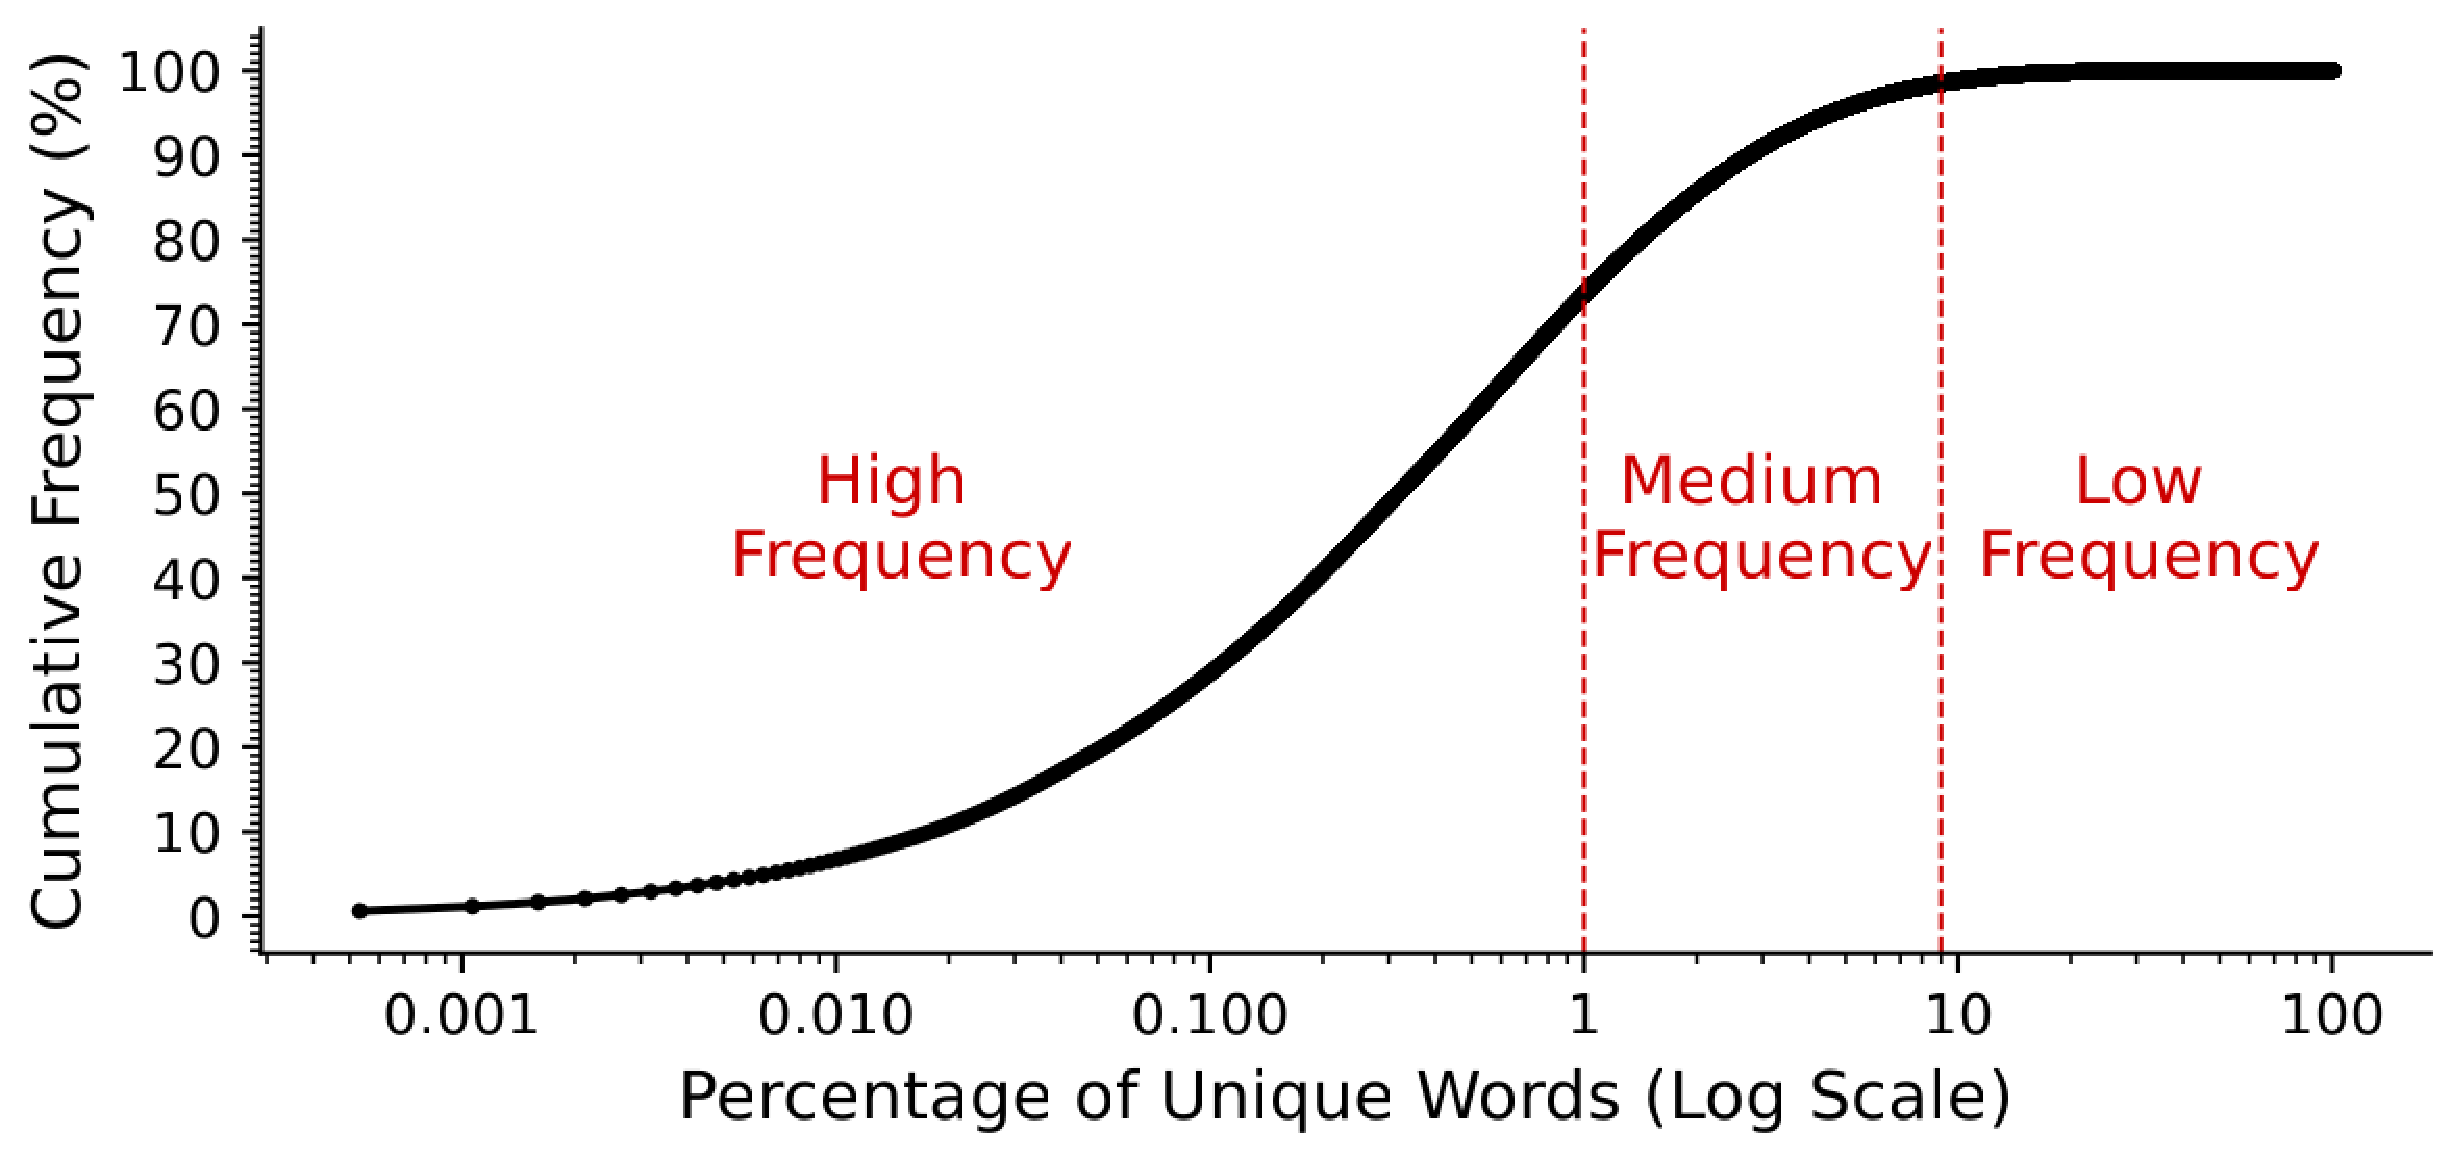
\includegraphics[width=0.5\linewidth]{flexheap/fig/method/words_freq.pdf}
	\caption{Distribution of words by their exact frequency in the dataset used for Lucene microbenchmarks.}
	\label{fig:words_freq}
\end{figure}

We use a \SI{300}{GB} real-world dataset~\cite{commoncr84:online} that contains 52.6 billion words.
To build our queries, we first perform a word count to determine the exact number of frequency for each word.
Then, we remove stop-words, single-character words, and non-English words.
Figure~\ref{fig:words_freq} shows the cumulative distribution of words (after selection) by their exact frequency.

Based on these counts, we classify the words into three categories: high-frequency, medium-frequency, and low-frequency.
The top 1\% of words are classified as high-frequency, accounting for 80\% of total occurrences.
In contrast, 91\% of words are low-frequency, representing only 1\% of total occurrences.
The remaining words fall into the medium-frequency category.
These frequency thresholds help us simulate different levels of I/O load during query processing.
High-frequency words appear in more documents within the Lucene index, resulting in higher I/O due to the need to access more documents.
In contrast, low-frequency words generate less I/O.
By using these frequency categories, we can effectively simulate varying I/O loads and analyze their impact on query performance.

We create small and large queries that fetch the top 50 or top \num{500000} results, respectively.
Unlike small queries, large queries require more memory in the managed heap because they create more memory pressure.
On the one hand, the frequency dimension (i.e., high, medium, and low) affects I/O.
Conversely, the number of results affects pressure in the managed heap.
Table~\ref{tab:lucene_queries} shows the performance implications of DRAM allocation between the managed heap and the I/O cache under different query loads.
Note that we omit running low-frequency queries with \num{500000} results since their results are typically fewer than 1000.

% \input{flexheap/tab_lucene_queries}
%
% \input{flexheap/tab_lucene_mixes}

\setlength\heavyrulewidth{1pt}
\begin{table}[h]
	\centering
	\begin{minipage}{0.55\textwidth}
		\centering
		\caption{Description of the mixes of Lucene queries.}
		\resizebox{\textwidth}{!}{%
			\begin{tabular}{l|ccc|cc}
				\textbf{\begin{tabular}[c]{@{}l@{}}\end{tabular}}                   & \multicolumn{3}{c|}{\textbf{Top 50}}                          & \multicolumn{2}{c}{\textbf{Top 500,000}}                                                                                                                                                                                                                             \\ \cline{2-6}
				\textbf{\begin{tabular}[c]{@{}l@{}}\end{tabular}}                   & \textbf{\begin{tabular}[c]{@{}c@{}}High\\ (H50)\end{tabular}} & \textbf{\begin{tabular}[c]{@{}c@{}}Medium\\ (M50)\end{tabular}} & \textbf{\begin{tabular}[c]{@{}c@{}}Low\\ (L50)\end{tabular}} & \textbf{\begin{tabular}[c]{@{}c@{}}High\\ (H500k)\end{tabular}} & \textbf{\begin{tabular}[c]{@{}c@{}}Medium\\ (M500k)\end{tabular}} \\ \cline{2-6}
				\textbf{Number of Queries}                                          & 40,000                                                        & 80,000                                                          & 240,000                                                      & 300                                                             & 6,000                                                             \\
				\textbf{\begin{tabular}[c]{@{}l@{}}GC overhead (\%)\end{tabular}}   & 0.1                                                           & 0.2                                                             & 0.7                                                          & 21                                                              & 30                                                                \\
				\textbf{\begin{tabular}[c]{@{}l@{}}I/O per query (MB)\end{tabular}} & 30                                                            & 10                                                              & 3                                                            & 31                                                              & 2                                                                 \\
				\bottomrule
			\end{tabular}
		}
		\label{tab:lucene_queries}
	\end{minipage}
	\hfill
	\begin{minipage}{0.42\textwidth}
		\centering
		\caption{Configuration of Lucene workloads.}
		\resizebox{\textwidth}{!}{%
			\begin{tabular}{lcl}
				                            & \textbf{Id} & \textbf{Queries description} \\ \hline
				\multirow{1}{*}{Sequential} & M1          & H50-M500k-L50-H500k-M50      \\ \hline
				\multirow{3}{*}{Concurrent} & M2          & H50-M500k-H500k              \\
				                            & M3          & M50-M500k-H500k              \\
				                            & M4          & L50-M500k-H500k              \\ \hline
			\end{tabular}
		}
		\label{tab:lucene_workloads}
	\end{minipage}
\end{table}

As shown in Table~\ref{tab:lucene_workloads}, we construct four experimental configurations using the query categories described in Table~\ref{tab:lucene_queries}.
%
M1 executes queries of different types sequentially without mixing them.
All queries in H50 (high frequency top 50 results) run before any of the M500k queries, etc.
Queries in each type are executed from 32 clients.
%
For the last three configurations (concurrent), we use 16 clients to execute the small queries, and another 16 clients execute the large queries concurrently.
The large queries arrive in batches based on a Poisson distribution, which aims to reflect the random nature of real-world query arrival rates.
This approach helps us understand how the system handles a diverse and concurrent query load, reflecting real-world usage more accurately.
To investigate future setups where the index size is significantly larger than the available DRAM, we use two different DRAM budgets: one where the DRAM budget equals 5\% and another where it equals 10\% of the index size as stored on the disk.
We allow OpenJDK ergonomics to set up the number of STW and concurrent GC threads.

\paragraph{\textbf{Baselines}}
We compare \flexheapName{} against two classes of dynamic heap resizing: G1 (GC-based) and VG1 (occupancy-based, time-driven).
To compare against the latest G1 heap resizing mechanism, we port its resizing policy from OpenJDK 26 to OpenJDK 21.
VG1 remains unchanged across JDK versions.
For Elasticsearch, we follow the official guidelines~\cite{elasticsearch:guidelines} and cap G1 at 50\% of DRAM (G1-50), leaving the remainder to the I/O cache.
We omit G1-90 from the main Elasticsearch evaluation because, as shown in Section~\S~\ref{flexheap:sec:motiv}, it consistently results in longer execution time than G1-50.
Accordingly, G1-50 serves as the strongest G1 baseline recommended for deployment.
For Spark, we cap the maximum heap at 75\% of DRAM (G1-75), following the guidelines of Spark 4.0.1~\cite{spark:guidelines}.
We configure VG1 to trigger a \flexheapGC{} every second to resize the heap and release memory back to the OS, as in prior work~\cite{bruno:resize}.
In Elasticsearch, VG1’s maximum heap is capped at 90\% of the DRAM budget, whereas in Spark it is capped at 75\%.
\flexheapName{} uses the same maximum heap cap as VG1 for each workload.
We note that in Spark, all systems use the same maximum heap cap, therefore, any differences are due to the heap resizing policy.
